% @out_file dokumentace.tex
% @author Štěpán Faragula
% @brief Dokumentace semestrální práce z předmětu KIV/ZOS.
% @version 1.0
% @date 2024-03-01

% Document
\documentclass[12pt]{report}

% Čeština
\usepackage[utf8]{inputenc}
\usepackage[T1]{fontenc}
\usepackage[czech]{babel}

% Formát dokumentu
\usepackage{amsmath}
\usepackage{caption}
\usepackage{textcomp}
\usepackage{xspace}
\usepackage{parskip}
\usepackage[hidelinks]{hyperref}

% Graphics
\usepackage{graphicx}
\graphicspath{{img/}}
\usepackage{fancyvrb}
\usepackage[
left=30mm, 
right=30mm, 
top=30mm, 
bottom=30mm,
]{geometry}

% Vychytávky
\usepackage{lipsum}								% Lorem impsum
\usepackage{pdflscape}							% Landscape
\usepackage{menukeys}							% Klavesy
\usepackage{algorithm}							% Algoritmus
\usepackage[noend]{algpseudocode}				% Pseudokod
\usepackage{dirtree}							% Adresarova struktura
												% Tabulky pomoci https://www.tablesgenerator.com/

\newcommand\indentt[1]{						
	\setlength\parindent{5mm}
	#1
	\setlength\parindent{0mm}
}	

% Begin
\begin{document}
	
	% Titulní strana
	\begin{titlepage}
		\centering
		\Large
		
		
\includegraphics[width=.7\textwidth]{fav}
		
		\vspace{15mm}
		{\Huge\bfseries Souborový systém založený na i-uzlech}
		
		\vspace{5mm}
		{\LARGE Katedra informatiky a výpočetní techniky}
		
		{\LARGE Semestrální práce z předmětu KIV/ZOS}
		
		\vfill
		\raggedright
		Štěpán Faragula\\
		A21B0119P\\
		farag844@students.zcu.cz
		\hfill 
		\today
	\end{titlepage}
	
	
	% Obsah
	\tableofcontents


	% Zadání	
	\chapter{Zadání}
	Tématem semestrální práce bude práce se zjednodušeným souborovým systémem založeným na i-uzlech. Vaším cílem bude splnit několik vybraných úloh.
		
	Program bude mít jeden parametr a tím bude název Vašeho souborového systému. Po~spuštění bude program čekat na zadání jednotlivých příkazů s minimální funkčností viz~níže (všechny soubory mohou být zadány jak absolutní, tak relativní cestou):
	
	\begin{enumerate}
		\item Zkopíruje soubor s1 do umístění s2
		\\ \texttt{cp s1 s2}
		\\
		\item Přesune soubor s1 do umístění s2, nebo přejmenuje s1 na s2
		\\ \texttt{mv s1 s2}
		\\
		\item Smaže soubor s1
		\\ \texttt{rm s1}
		\\
		\item Vytvoří adresář a1
		\\ \texttt{mkdir a1}
		\\
		\item Smaže prázdný adresář a1
		\\ \texttt{rmdir a1}
		\\
		\item Vypíše obsah adresáře a1
		\\ \texttt{ls a1}
		\\ \texttt{ls}
		\\
		\item Vypíše obsah souboru s1
		\\ \texttt{cat s1}
		\\
		\item Změní aktuální cestu do adresáře a1
		\\ \texttt{cd a1}
		\\
		\item Vypíše aktuální cestu
		\\ \texttt{pwd}
		\\
		\item Vypíše informace o souboru/adresáři s1/a1 (v jakých clusterech se nachází)
		\\ \texttt{info a1}
		\\ \texttt{info s1}
		\\
		\item Nahraje soubor s1 z pevného disku do umístění s2 ve vašem FS
		\\ \texttt{incp s1 s2}
		\\
		\item Nahraje soubor s1 z vašeho FS do umístění s2 na pevném disku
		\\ \texttt{outcp s1 s2}
		\\
		\item Načte soubor z pevného disku, ve kterém budou jednotlivé příkazy, a začne je~sekvenčně
		vykonávat. Formát je 1 příkaz na 1 řádek
		\\ \texttt{load s1}
		\\
		\item Formát souboru, který byl zadán jako parametr při spuštení programu na souborový systém dané velikosti. Pokud už soubor nějaká data obsahoval, budou přemazána. Pokud soubor neexistoval, bude vytvořen.
		\\ \texttt{format 600MB}
		\\
		\item Vytvoří hardlink na soubor s1 s názvem s2. Dále se s ním pracuje očekávaným způsobem, tedy např. cat s2 vypíše stejný obsah jako cat s1.
		\\ \texttt{ln s1 s2}
		\\
	\end{enumerate}
	
	Budeme předpokládat korektní zadání syntaxe příkazů, nikoliv však sémantiky (tj. např. cp s1 zadáno nebude, ale může být zadáno cat s1, kde s1 neexistuje).
		
	Každý název bude zabírat právě 12 bytů (do délky 12 bytů doplníme '\texttt{\textbackslash0}').
	
	Dále předpokládáme, že adresář se vždy vejde do jednoho clusteru (limituje nám počet položek v adresáři).
		
		
	% Návrh řešení
	\chapter{Struktura souborového systému}
	Souborový systém založený na i-uzlech reprezentuje každý soubor či adresář jedním i-uzlem (anglicky index node). Jedná se o strukturu obsahující metadata a reference na datové bloky souboru. Tyto odkazy jsou rozděleny na přímé a nepřímé, kde přímé ukazují na datový blok s obsahem souboru a nepřímé na čísla bloků ve kterých jsou uloženy data souboru. Nepřímé odkazy mohou být víceúrovňové, kde každá úroveň víc bude ukazovat na další nepřímé odkazy. V této práci obsahuje každý i-uzel 5 přímých odkazů, 1 nepřímý 1. úrovně a 1 nepřímý 2. úrovně.
	
	Adresáře ukládají na datový blok dvojici názvu souboru a index i-uzlu pro každý soubor co obsahují. Dále obsahují dvojici reprezentující sebe sama '\texttt{.}' a rodičovský adresář '\texttt{..}'.
	
	Celý souborový systém pracuje s přiděleným místem na disku. V případě semestrální práce je tento prostor simulován textovým souborem zadané velikosti. Aby mohl být systém snadno uložen a načten, zapisuje data do souboru v určitém pořadí, které je~znázorněno na obrázku \ref{fig:struktura}. Význam jednotlivých bloků je následující:
	
	\begin{figure}
		\centering
		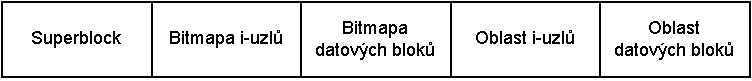
\includegraphics[width=1\textwidth]{struktura}
		\caption{Struktura souborového systému}
		\label{fig:struktura}
	\end{figure}
	
	\begin{itemize}
		\item Superblock = metadata souborového systému
		\item Bitmapa i-uzlů = zobrazuje volné/zabrané indexy i-uzlů
		\item Bitmapa datových bloků = zobrazuje volné/zabrané indexy datových bloků
		\item Oblast i-uzlů = zde se ukládají datové struktury i-uzlů
		\item Oblast datových bloků = zde se ukládají konkrétní data souborů/adresářů
	\end{itemize}


	% Programátorská dokumentace
	\chapter{Programátorská dokumentace}
	Počet i-uzlů je pevně nastaven na 1024, je tak nejlépe využit paměťový prostor příslušné bitmapy. Velikost datového bloku je nastavena na 512 bytů. Vzhledem k počtu referencí co může i-uzel obsahovat je maximální velikost souboru zhruba 8,5 MB. Jelikož názvy souborů jsou omezeny na 12 znaků a pro reference je použit 32bitový integer, datový blok adresáře může obsahovat maximálně 32 odkazů na datové bloky.
	
	Práce je vytvořena v jazyce C/C++. Požadavky uživatele jsou vyhodnocovány v nekonečné smyčce pomocí funkce \texttt{parse\_input()}. Struktura programu je rozdělena mezi několik souborů obsahující třídy a funkce zabývající se určitou problematikou. Ve zkratce se jednotlivé soubory zabývají následujícím:
	\begin{itemize}
		\item \texttt{Constants} - konstanty programu
		\item \texttt{Main} - spouští souborový systém, přijímá vstup uživatele
		\item \texttt{InputParser} - zpracovává vstup, předává data k vykonání požadavku
		\item \texttt{FileSystem} - obsahuje jednotlivé příkazy které uživatel volá, vykonává operace nad virtuálním souborovým systémem
		\item \texttt{Superblock} - metadata souborového systému
		\item \texttt{Bitmap} - bitmapa volných indexů
		\item \texttt{IndexNode} - i-uzel
		\item \texttt{Directory} - datový blok adresáře
		\item \texttt{DirectoryItem} - položka adresáře
		\item \texttt{ReferenceBlock} - datový blok obsahující odkazy na jiné datové bloky
	\end{itemize}

		
	% Uživatelská příručka
	\chapter{Uživatelská příručka}
	Pro překlad a spuštění aplikace je nutné mít nainstalované programy \texttt{g++}, \texttt{cmake} a~\texttt{make}. Program očekává jeden parametr při spuštění, a to cestu k souboru obsahující data souborového systému. Příklad spuštění je následující:
	
	\indentt{
		\texttt{./ZOS\_Semestralka myFileSystem}
	}
	
	Pokud soubor existuje, zkusí data načíst. Pokud ne, vyžaduje od uživatele o zavolání příkazu \texttt{format}, který následně soubor vytvoří. Aplikace se řádně ukončí příkazem \texttt{exit} či zasláním signálu \texttt{SIGINT}.
	
	Tabulka \ref{tab:tabulka} obsahuje všechny příkazy, které lze nad souborovým systémem vykonat.
	\begin{table}[H]
		\begin{tabular}{|l|l|}
			\hline
			\texttt{cp s1 s2} & Zkopíruje soubor s1 do umístění s2 \\ \hline
			\texttt{mv s1 s2} & Přesune soubor s1 do umístění s2, nebo přejmenuje s1 na s2 \\ \hline
			\texttt{rm s1} & Smaže soubor s1 \\ \hline
			\texttt{mkdir a1} & Vytvoří adresář a1 \\ \hline
			\texttt{rmdir a1} & Smaže prázdný adresář a1 \\ \hline
			\texttt{ls a1} & Vypíše obsah adresáře a1 \\ \hline
			\texttt{cat s1} & Vypíše obsah souboru s1 \\ \hline
			\texttt{cd a1} & Změní aktuální cestu do adresáře a1 \\ \hline
			\texttt{pwd} & Vypíše aktuální cestu \\ \hline
			\texttt{info a1} & Vypíše informace o souboru s1 \\ \hline
			\texttt{incp s1 s2} & Nahraje soubor s1 z pevného disku do umístění s2 ve vašem FS \\ \hline
			\texttt{outcp s1 s2} & Nahraje soubor s1 z vašeho FS do umístění s2 na pevném disku \\ \hline
			\texttt{load s1} & Načte soubor s příkazy a začne je sekvenčně vykonávat \\ \hline
			\texttt{format 600MB} & Připraví strukturu souborového systému o dané velikosti \\ \hline
			\texttt{ln s1 s2} & Vytvoří hardlink na soubor s1 s názvem s2 \\ \hline
			\texttt{exit} & Řádně ukončí aplikaci \\ \hline
		\end{tabular}
		\caption{Dostupné příkazy souborového systému}
		\label{tab:tabulka}
	\end{table}
	

	% Závěr
	\chapter{Závěr}
	Souborový systém založený na i-uzlech splňuje všechny požadavky zadání. Umožňuje základní manipulaci se soubory a adresáři, kterou lze od souborového systému očekávat. Neumožňuje však vytvářet a upravovat obsah souborů. Tato funkcionalita by vyžadovala rozhraní textového editoru, což by bylo nad rámec řešení semestrální práce. 
	
	Možné vylepšení by mohlo být v hledání volného místa v bitmapě, jelikož nyní se~vyhledává jedno po druhém nezávisle na sobě a u načítání velkých souborů tento přístup způsobuje zpomalení. Namísto nezávislého naivního hledání by se bitmapa mohla prohledat pouze jednou a vrátit seznam s potřebným počtem volných míst.

\end{document}
